\section{Comparison with related work} \label{sec:dpl}

Constants, variables, reference markers: $\mathsf{C}, \mathsf{V}, \mathsf{M}$

model: $\mathscr{M} = \langle D, \mathcal{I}\, \rangle$

left contexts : $\env = D^{\mathsf{M}}$

continuations : $\cont = 2^\env$ 

nota: a tdl term may contain ref. markers (this stands for $\sel{}$)

\begin{align*}
\dplsem{\eta}{\app{\app{\app{R}{t_1}}{\ldots}}{t_n}} &= 
\{\langle g,h\rangle  :
h=g \,\wedge\, 
\langle 
\llbracket t_1 \rrbracket_{\eta,g},
\dots,
\llbracket t_n \rrbracket_{\eta,g}
\rangle \in \mathcal{I}(R)
\}
\\
\dplsem{\eta}{\conj{P}{Q}} &= 
\{\langle g,h\rangle  : 
\equant{k}{
\langle g,k\rangle\in \dplsem{\eta}{P}
\,\wedge\,
\langle k,h\rangle\in \dplsem{\eta}{Q}
}\}
\\
\dplsem{\eta}{\nega{P}} &=
\{\langle g,h\rangle  : 
h=g \,\wedge\, 
\uquant{k}{\langle g,k \rangle\not\in\dplsem{\eta}{P}}
\}
\\
\dplsem{\eta}{\equant{\mathbf{i}}{P}} &=
\{\langle g,h\rangle  : 
\equant{k}{
k[\mathbf{i}]g \,\wedge\,
\langle k,h \rangle \in \dplsem{\eta}{P}
}\} 
\end{align*}

\begin{align*}
\synlift{c}_e &= c\\
\synlift{x}_e &= x\\
\synlift{\mathbf{i}}_e &= \app{\mathsf{sel}_i}{e}\\
\end{align*}

\begin{align*}
\synlift{\app{\app{\app{R}{t_1}}{\ldots}}{t_n}} &= 
\abs{e\phi}{\conj{
\app{\app{\app{R}{
\synlift{t_1}_e
}}{\ldots}}{
\synlift{t_n}_e}
}{\app{\phi}{e}}}
\\
\synlift{\conj{P}{Q}} &= 
\dconj{\synlift{P}}{\synlift{Q}}
\\
\synlift{\nega{P}} &= \dnega{\synlift{P}}
\\
\synlift{\equant{\mathbf{i}}{P}} &=
\dynexists_{\mathbf{i}} x.\,\synlift{P[\mathbf{i}{:=}x]}
\end{align*}

\begin{align*}
\tdlsem{\eta}{\app{\app{\app{R}{t_1}}{\ldots}}{t_n}} &= 
\{\langle g,H\rangle   :
g \in H \, \wedge \,
\langle 
\llbracket t_1 \rrbracket_{\eta,g},
\dots,
\llbracket t_n \rrbracket_{\eta,g}
\rangle \in \mathcal{I}(R)
\}
\\
\tdlsem{\eta}{\dconj{P}{Q}} &= 
\{\langle g,H\rangle  :
\langle g, 
\{h : \langle h, H\rangle \in \tdlsem{\eta}{Q}\}
\rangle\in\tdlsem{\eta}{P}
\}
\\
\tdlsem{\eta}{\dnega{P}} &=
\{\langle g,H\rangle  :
g \in H \, \wedge \,
\langle g,\env\rangle\not\in \tdlsem{\eta}{P}
\}
\\
\tdlsem{\eta}{\dynexists_{\mathbf{i}} x.\, P} &=
\{\langle g,H\rangle  :
\equant{a}{\langle g[\mathbf{i}{:=}a],H\rangle\in\tdlsem{\eta[x{:=}a]}{P}}
\} 
\end{align*}

$$
\semlift{\mathrm{R}} = \{\langle a,B\rangle : 
\equant{b}{\conj{b\in B}{\langle a,b\rangle\in R}}\}
$$



\begin{lemma}\label{substlemma1}
Let $t$ be a term, and let $x$ be a variable that does not occur in $t$.
For all reference marker $\mathbf{i}$, all assignment $g$, and all valuation
$\eta$, the following holds:
$$
\llbracket t \rrbracket_{\eta,g} =
\llbracket t[\mathbf{i}{:=}x] \rrbracket_{\eta[x{:=}(\app{g}{\mathbf{i}})],g}
$$
\begin{proof}
If $t$ is a constant or a reference marker different from $\mathbf{i}$,
the result is immediate.
If $t$ is a variable $y$, we have that $y\not= x$. Consequently,
$\app{\eta}{y} = \app{\eta[x{:=}(\app{g}{i})]}{y}$.
Finally, if $t$ is $\mathbf{i}$, we have
$\llbracket \mathbf{i} \rrbracket_{\eta,g} =
\app{g}{\mathbf{i}} = 
\app{\eta[x{:=}(\app{g}{i})]}{x} = 
\llbracket x \rrbracket_{\eta[x{:=}(\app{g}{\mathbf{i}})],g} =
\llbracket\mathbf{i}[\mathbf{i}{:=}x] \rrbracket_{\eta[x{:=}(\app{g}{\mathbf{i}})],g}
$.
\end{proof}
\end{lemma}

\begin{lemma}\label{substlemma2}
Let $P$ be a DPL formula, and let $x$ be a variable that does not occur in $P$.
For all reference marker $\mathbf{i}$, all pair of assignments 
$\langle g, h \rangle$, and all valuation
$\eta$, the following holds:
$$
\langle g,h\rangle \in \dplsem{\eta}{P}
\mbox{ if and only if }
\langle g,h\rangle \in 
\dplsem{\eta[x{:=}(\app{g}{\mathbf{i}})]}{P[\mathbf{i}{:=}x]}
$$
\begin{proof}
A straightforward induction on the structure of $P$, using 
Lemma~\ref{substlemma1} for the base case.
\end{proof}
\end{lemma}

\begin{lemma}\label{commutlemma}
Let $P$ be a DPL formula, and $\eta$ be a valuation.
Then, the following holds:
$$
\semlift{\dplsem{\eta}{P}} = \tdlsem{\eta}{\synlift{P}}
$$
\begin{proof}
Xxx.
\end{proof}
\end{lemma}

\begin{proposition}
Let $P$ be a DPL formula, and $g$ be an assignment.  
Then, $\dplvalid{g}{P}$
if and only if
$\tdlvalid{g}{P}$.
\begin{proof}
Xxx.
\end{proof}
\end{proposition}




----------------------------------------------

DPL, at least as it is presented in~\cite{GroenendijkStokhof:1991:Dynamic-Predicate-Logic} does not provide a translation from natural language to the language of DPL. In contrast, this dissertation is focused exactly on providing a translation from natural language to the language of continuation based-dynamic logic. This makes it impossible to make a direct comparison between DPL and {\GLex} (as well as its predecessors {\GN} and {\GL}). Nevertheless, it is still possible to compare the frameworks by defining certain translations between their different levels. Since, among {\GN}, {\GL} and {\GLex}, the closest to DPL w.r.t. expressive power is {\GN}, translations between {\GN} and DPL are defined subsequently.

Consider Figure~\ref{DPLscheme}. The missing translation $\ntodpl$ of natural language into the language of DPL is represented by the dashed arrow. The translation $\ntodl$ of natural language into the language $\langDL$ of continuation-based dynamic logic is represented by the green arrow.
 \begin{figure}[h!]
  \centering
    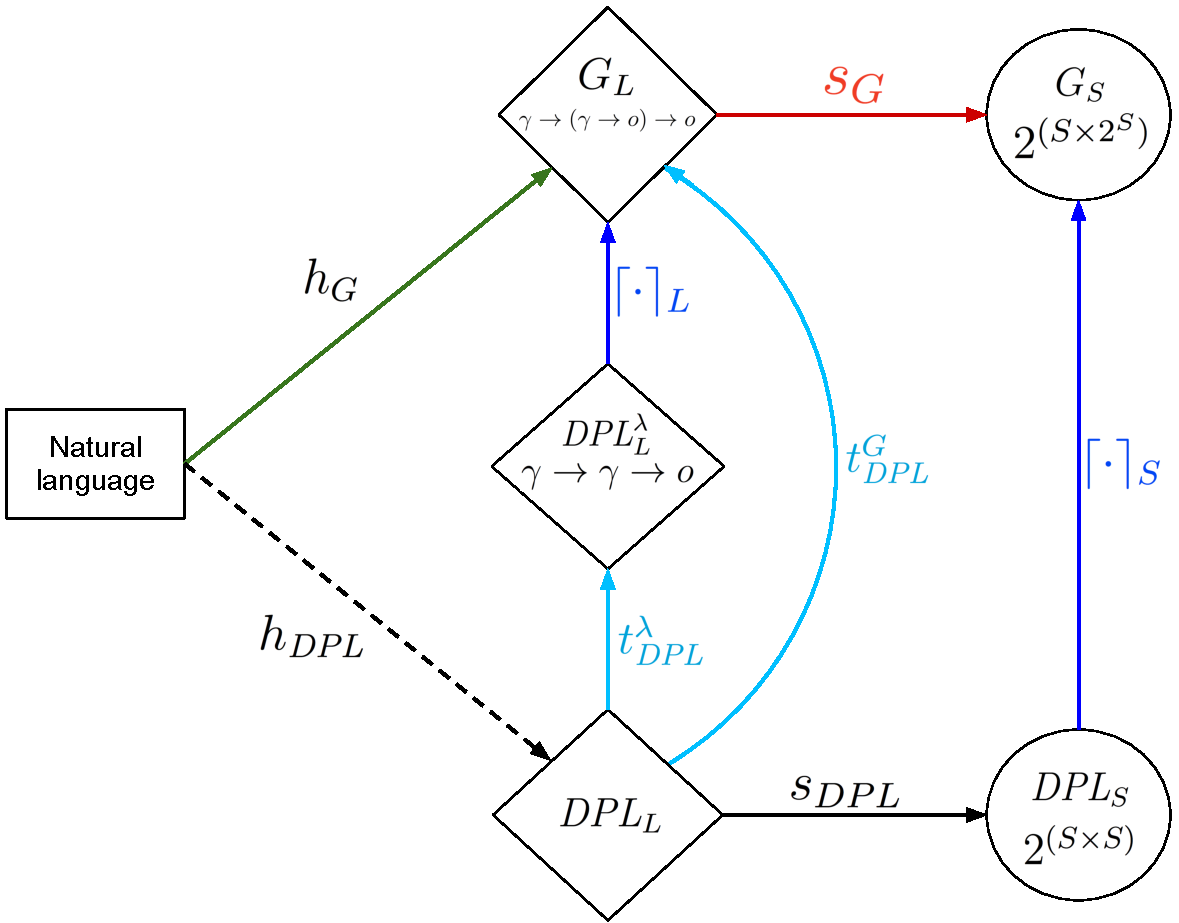
\includegraphics[width=1\textwidth]{images/DPLscheme.pdf}
      \caption{Comparison between DPL and {\GN}.} \label{DPLscheme}
\end{figure}

What Groenendijk and Stokhof~\cite{GroenendijkStokhof:1991:Dynamic-Predicate-Logic} define is a translation $\dpltos$ of the language of DPL into binary relations on states $\statesDPL$. This translation is illustrated with the black solid arrow.

There are two possible ways to compare DPL and {\GN}. One possibility is to define a translation $\dltos$ (red arrow) of the language of {\GN} into relations on states $\statesDL$ and to compare  $\statesDL$ with $\statesDPL$. Another possibility is to define a translation $\dplstodpll$ (shorter light blue arrow) of the language $\langDPL$ of DPL into a new language $\newDPL$ and to compare $\newDPL$ with the language  $\langDL$ of {\GN}. These two comparisons are presented in more details below.


\subsubsection{Comparison 1}

DPL interprets propositions as binary relations on states and its semantics is defined as the following translation from $\langDPL$ to $\statesDPL$ (solid black arrow):
\begin{definition}[Translation $\dpltos$] Let $A, B$ and $P$ be terms in $\langDPL$ of type $o$. Let $h, g$ and $k$ be assignments of values to variables (a.k.a. states). Translation $\dpltos:  \langDPL \rightarrow \statesDPL$ is defined as follows:
\begin{align*}
\mdpltos{A} = \ & \{ \langle g , h \rangle \ | \ h = g \land h  \models A \} \\
\mdpltos{\neg P} = \ & \{ \langle g , h \rangle \ | \ h = g \land \neg ( \exists k.  \ \langle h, k \rangle \in  \mdpltos{P} ) \} \\
\mdpltos{A \land B} = \ & \{ \langle g , h \rangle \ |  \ \exists k. \ \langle g, k \rangle \in  \mdpltos{A}  \land   \langle k, h \rangle \in  \mdpltos{B}  \} \\
\mdpltos{\exists i. P} = \ & \{ \langle g , h \rangle \ |  \ \exists k.  \  k [i] g \land  \langle k, h \rangle \in  \mdpltos{P} \} 
\end{align*}
\end{definition}
\noindent Thus, for every proposition $P$, $\mdpltos{P}$ is in $2^{(S \times S)}$.
%

\noindent A similar translation $\dltos$ (red arrow) of propositions in $\langDL$ into relations defined on states can be defined:
\begin{definition}[Translation $\dltos$] Let $S$, the set of states, be the semantic domain that interprets $\gamma$. The translation $\dltos: \langDL \rightarrow \statesDL$ is defined as follows:
\begin{align*}
\mdltos{A} = \ & \{ \langle g , H \rangle \ | \ g \in H \land g \models A \} \\
\mdltos{\n2 P} = \ & \{ \langle g , H \rangle \ | \ g \in H \land \langle g, S \rangle \notin \mdltos{P} \} \\
\mdltos{A \cnj2 B} = \ & \{ \langle g , H \rangle \ | \ \langle g , \{ h \ | \ \langle h, H \rangle \in \mdltos{B} \} \rangle \in \mdltos{A} \} \\
\mdltos{\ex2_i x. P} = \ & \{ \langle g , H \rangle \ | \ \exists x. \langle (x,i)::g ,  H \rangle \in \mdltos{P} \} 
\end{align*}
\end{definition}
Note that  $\dltos$ interprets propositions not just as relations between states, but as relations betweens states and sets of states: for each proposition $P$, $\mdltos{P}$ is in  $2^{(S \times 2^S)}$. Therefore, $\dltos$ is richer than $\dpltos$ and avoids existentially quantified states and equality relations on states by using set inclusion.  Moreover, there exists a canonical embedding (larger blue arrow) of $\statesDPL$ into $\statesDL$:
\begin{definition}[Embedding of $\statesDPL$ into $\statesDL$] Let $R$ be set of pair of states (in $2^{(S \times S)}$) in $\statesDPL$, the embedding $\dplstodls$ of $\statesDPL$ into $\statesDL$ is as follows: 
\begin{align}
\mdplstodls{R} \defeq \ & \{  \langle g, H \rangle \ | \ \exists h. \ h \in H \land \langle g, h \rangle \in R  \} \notag
\end{align}
$\mdplstodls{R}$  is in $2^{(S \times 2^S)}$.
\end{definition}
Note that there is a correspondence between types constructed from $\gamma$ and $o$ and sets constructed from $S$ and the cross product powerset operations:
\begin{align}
 [\gamma ] \approx \ & S \notag \\
 [\alpha_1 \rightarrow \alpha_2 \rightarrow  \dots \rightarrow \alpha_n \rightarrow o] \approx \ & 2^{[\alpha_1] \times [\alpha_2] \times \dots \times [\alpha_n]} \notag
\end{align}
Consequently, the type $(\gamma \rightarrow (\gamma \rightarrow o) \rightarrow o )$ corresponds to the set $2^{(S \times 2^S)}$.

 The following translation $\dpltodl$ (longer light blue arrow) of  $\langDPL$ to  $\langDL$ can be defined:
\begin{definition}[Translation $\dpltodl$] Let $A, B$ and $P$ be propositions. The translation $\dpltodl: \langDPL \rightarrow \langDL$ is defined as follows:
\begin{align*}
 \mdpltodl{A}  = \ & A \\
 \mdpltodl{\neg P} = \ & \n2 \mdpltodl{P} \\
 \mdpltodl{ A \land B} = \ & \mdpltodl{A} \cnj2 \mdpltodl{B} \\ 
 \mdpltodl{\exists i. P} = \ & \ex2_i x. \mdpltodl{P}
\end{align*}
\end{definition}

\begin{theorem} \label{th:dplltodll} Let $P$ be a proposition. Then the following equivalence holds:
\begin{align}
 \mdplstodls{ \mdpltos{P}} = \mdltos{\mdpltodl{P}} \notag
\end{align}
by postulating
\begin{align}
g [i] h \ \  \text{iff} \  \ \exists x. (h = (x,i)::g) \notag
\end{align}
\end{theorem}
\begin{proof} The proof is by induction on the structure of $P$.
\end{proof}

By Theorem~\ref{th:dplltodll}, transforming $\langDPL$ to $\langDL$ and interpreting the result in $\statesDL$ according to $\dltos$ is equivalent to DPL's original semantics. 

\subsubsection{Comparison 2}

Each proposition $A$ in $\langDPL$ can be translated into a term of type $(\gamma \rightarrow \gamma \rightarrow o)$ in $\newDPL$ in a way that reflects the semantics of DPL. The translation is given by the following definition:
\begin{definition}[Translation $\dplstodpll$] Let $T$ of type $o$ be an atomic proposition, $P, A$, and $B$ of type $o$ be propositions, $g,h$ and $k$ be variables of type $\gamma$. The translation $\dplstodpll:\langDPL \rightarrow \newDPL$ is defined as follows:
\begin{subequations}
\begin{align}
 \mdplstodpll{T} \defeq \ & \lambda gh. \  h = g \land T \label{eq:DPLL:atom} \\
 \mdplstodpll{\neg P} \defeq \ & \lambda gh. \ h = g \land \neg (\exists k. \mdplstodpll{P} h k) \label{eq:DPLL:neg} \\
 \mdplstodpll{A \land B} \defeq \ & \lambda gh.  \ \exists k. \ \mdplstodpll{A} g k  \land \mdplstodpll{B} k h  \label{eq:DPLL:and} \\
 \mdplstodpll{\exists x. P} \defeq \ & \lambda gh.  \ \exists k. \  k [ x] g \land \mdplstodpll{P} k h \label{eq:DPLL:exist} 
\end{align}
\end{subequations}
\end{definition}

\noindent The resulting language $\newDPL$ can be compared with $\langDL$. 

Note that $\newDPL$ has the existential quantifier in the definitions of negation~\eqref{eq:DPLL:neg} and conjunction~\eqref{eq:DPLL:and} and a subterm with equality in the definitions of the atomic proposition~\eqref{eq:DPLL:atom} and negation~\eqref{eq:DPLL:neg}. DPL uses these existential quantifications and equalities in order to constraint the pairs of states that represent the final interpretation. Because of that, the final interpretation in $\newDPL$ would have chains of equalities of the form $\dots \land g = g' \land  \dots  \land g'=g'' \land  \dots   $ and some deductive reasoner would be required for establishing the final interpretation of a sentence.
 In {\GN}, however, there is no need for this kind of equalities and existential quantification.  All necessary restrictions that natural language poses on a model are interpreted using $\beta$-reduction only.

A canonical embedding (smaller blue arrow) of $\newDPL$ into $\langDL$ can be defined:
\begin{definition}[Embedding of $\newDPL$ into $\langDL$] Let $A$ be a term of type $(\gamma \rightarrow \gamma \rightarrow o)$ in $\newDPL$, the embedding $\dpllstodl$  of $\newDPL$ into $\langDL$ is as follows:
\begin{align}
\mdpllstodl{A} \defeq \lambda e \phi. \exists e'.  \ \phi \ e' \land  A \ e \ e'  \notag
\end{align}
$\mdpllstodl{A}$ is of type $(\gamma \rightarrow (\gamma \rightarrow o) \rightarrow o)$.
\end{definition}


\begin{theorem} Let $A, B$ and $P$ be terms of type $o$ in $\langDPL$. Then the following logical equivalences hold:
\begin{align*}
\mdpllstodl{\mdplstodpll{A}} \logeq \ & \tr{A} \notag \\
\mdpllstodl{ \mdplstodpll {\neg P} } \logeq \ & \n2  \mdpllstodl{ \mdplstodpll {P} } \notag \\
\mdpllstodl{ \mdplstodpll { A \land B} } \logeq \ &  \mdpllstodl{ \mdplstodpll { A } }  \cnj2 \mdpllstodl{ \mdplstodpll {B} }
\end{align*}
\end{theorem}
\begin{proof}
The proof is by induction on the structure of terms.
\end{proof}

\noindent An analogous logical equivalence does not hold, however, for the existential quantifier: $\mdpllstodl{ \mdplstodpll { \exists x. P} } $ reduces to ~\eqref{eq:DPL:exist1} and $\ex2 \mdpllstodl{ \mdplstodpll {P} } $ reduces to~\eqref{eq:DPL:exist2}:
\begin{align}
\mdpllstodl{ \mdplstodpll { \exists x. P} } = \ & \lambda e \phi. \ \exists e'.  \ \phi \ e' \land \exists k. \ k [x] e \land \mdpllstodl{ \mdplstodpll {P} } \  k \ e'  \label{eq:DPL:exist1} \\
\ex2 \mdpllstodl{ \mdplstodpll {P} } = \ & \lambda e \phi.  \ \exists e'.  \ \phi \ e' \land  \exists x. \ \mdpllstodl{ \mdplstodpll {P} } \ (x::e) \ e'  \label{eq:DPL:exist2} 
\end{align}
Nevertheless, terms~\eqref{eq:DPL:exist1} and~\eqref{eq:DPL:exist2} are similar from the point of view of constraining their interpretation in a model. Thus, the constraint in~\eqref{eq:DPL:exist1} that $k$ is interpreted as $e$ except for the values of $x$ is expressed in
~\eqref{eq:DPL:exist2} simply by explicit update of the context $e$ with $x$.
Note, moreover, that $x$ is a free variable in~\eqref{eq:DPL:exist1}, whereas~\eqref{eq:DPL:exist2} is a closed term. Therefore, interpretation~\eqref{eq:DPL:exist2} is advantageous over~\eqref{eq:DPL:exist1}.
 